\chapter{प्रोटीनों का संरचनात्मक जीवविज्ञान}\label{ch:b3:structural-biology}

मैक्स पेरुत्स ने हीमोग्लोबिन की संरचना पर काम 1937 में शुरू किया और उसे
1960 में प्रकाशित किया: आधे नैनोमीटर के \omterm{def:b3:structural-biology:methods}{विभेदन} पर यह देखने में बाईस
वर्ष कि डेढ़ सौ अमीनो अम्लों की चार शृंखलाएँ चार हीमों के चारों ओर कैसे
वलित होती हैं। हीमोग्लोबिन का कोई अणु स्वयं को कुछ मिलीसेकंडों में
वलित कर लेता है। इन दो तथ्यों के बीच इस अध्याय का विषय पड़ा है: किसी
प्रोटीन का आकार क्या है, अमीनो अम्लों की किसी शृंखला का एक आकार क्यों
होता है और दूसरा नहीं, वह इतने बड़े विकल्प-समूह में से वह आकार इतनी
तेज़ी से कैसे ढूँढ़ लेती है, जब वह ऐसा नहीं कर पाती तब क्या बिगड़ता है,
आकार देखे कैसे जाते हैं --- X-किरणों से, चुंबकीय अनुनाद से,
इलेक्ट्रॉनों से, और अब गणना से --- और कोई प्रोटीन अपना काम करने के लिए
आकारों के बीच कैसे चलता है, जिसमें हीमोग्लोबिन का तनी और शिथिल अवस्था
के बीच का स्विच तब से हर अन्यस्थानिक प्रोटीन का प्रतिरूप रहा है।

\section{किसी प्रोटीन की संरचना क्या है}

\begin{definition}[संरचना के स्तर]\label{def:b3:structural-biology:levels}
\index{द्वितीयक संरचना}\index{अल्फा कुंडली}\index{बीटा चादर}\index{तृतीयक संरचना}\index{प्रांत}\index{वलन}
\emph{प्राथमिक संरचना} अवशेषों का अनुक्रम है। \emph{द्वितीयक संरचना}
आधार-ढाँचे की स्थानिक नियमित संरूपता है, जो आधार-ढाँचे के कार्बोनिलों
और एमाइडों के बीच हाइड्रोजन बंधों से स्थिर होती है:
\emph{$\alpha$-कुंडली}, यानी प्रति फेरा $3.6$ अवशेषों वाला कोई
दक्षिणावर्त सर्पिल, जो प्रति अवशेष \qty{0.15}{nm} (प्रति फेरा
\qty{0.54}{nm}) उठता है और जिसमें हर कार्बोनिल चार अवशेष आगे के एमाइड
से बँधा है; और \emph{$\beta$-चादर}, जिसमें फैली हुई लड़ियाँ अगल-बगल
पड़ी रहती हैं, समांतर या प्रतिसमांतर, अपने पड़ोसियों से बँधी, और
पार्श्व-शृंखलाएँ चादर के ऊपर-नीचे बारी-बारी से निकलती हैं।
\emph{तृतीयक संरचना} किसी पूरी शृंखला का त्रिविम वलन है; उसके भीतर
\numrange{50}{250} अवशेषों की कोई सघन, स्वतंत्र रूप से वलित होने वाली
इकाई कोई \emph{प्रांत} है, और किसी प्रांत के द्वितीयक अवयवों का विन्यास
उसका \emph{वलन} है। \emph{चतुष्क संरचना} कई शृंखलाओं का जमाव है:
हीमोग्लोबिन का $\alpha_{2}\beta_{2}$। कोई \num{1300} वलन सारे ज्ञात
प्रांतों का हिसाब दे देते हैं, और उनमें से कुछ दर्जन --- रॉसमान वलन,
TIM पीपा, इम्यूनोग्लोबुलिन वलन --- सारे प्रोटीनों के बड़े अंश का:
प्रकृति वलनों को फिर-फिर काम में लेती है और उनके अनुक्रम बदलती रहती है।
\end{definition}

\begin{omfigure}
\begin{tikzpicture}
\begin{axis}[
  width=6.4cm, height=6.4cm,
  xmin=-180, xmax=180, ymin=-180, ymax=180,
  xlabel={$\phi$ (अंश)}, ylabel={$\psi$ (अंश)},
  xlabel style={font=\small}, ylabel style={font=\small},
  tick label style={font=\scriptsize}, xtick={-180,-90,0,90,180}, ytick={-180,-90,0,90,180},
  axis lines=box, grid=major, grid style={gray!25},
  clip=false,
]
% beta region
\fill[omDef!30] (axis cs:-180,90) rectangle (axis cs:-45,180);
\fill[omDef!30] (axis cs:-180,-180) rectangle (axis cs:-45,-150);
\node[font=\scriptsize, omDef!60!black] at (axis cs:-112,165) {$\beta$ लड़ियाँ};
% alpha R region
\fill[omThm!30] (axis cs:-160,-70) rectangle (axis cs:-45,0);
\node[font=\scriptsize, omThm!70!black] at (axis cs:-105,-58) {दक्षिणावर्त $\alpha$};
% alpha L region
\fill[omMeth!30] (axis cs:45,0) rectangle (axis cs:100,80);
\node[font=\scriptsize, omMeth!60!black, align=center] at (axis cs:72,40) {वामा-\\वर्त};
\addplot[only marks, mark=*, mark size=1pt, black] coordinates {(-57,-47)};
\node[font=\scriptsize, anchor=south west] at (axis cs:-52,-44) {$\alpha$: $(-57,-47)$};
\addplot[only marks, mark=*, mark size=1pt, black] coordinates {(-139,135)};
\node[font=\scriptsize, anchor=west] at (axis cs:-134,135) {प्रतिसमांतर $\beta$};
\end{axis}
\node[align=left, font=\scriptsize, anchor=west] at (7.0,3.0) {हर अवशेष के दोनों आधार-ढाँचा ऐंठन कोण,\\$\phi$ (N--C$_\alpha$ के परितः) और $\psi$ (C$_\alpha$--C\\के परितः), संकुलन-टकरावों से रँगे क्षेत्रों तक\\सीमित हैं। कोई कुंडली हर अवशेष को एक ही बिंदु\\पर रखती है; कोई लड़ी किसी दूसरे के पास।\\ग्लाइसीन, जिसकी कोई पार्श्व-शृंखला नहीं, दूर तक\\पहुँचता है; प्रोलीन, अपने वलय के कारण, $\phi = -60$ के पास बँधा है।};
\end{tikzpicture}

{\small रामचंद्रन आरेख। छायांकित क्षेत्र आधार-ढाँचा कोणों $\phi$ और
$\psi$ के वे संयोजन हैं जो संकुलन की दृष्टि से अनुमत हैं; दक्षिणावर्त
$\alpha$-कुंडली और $\beta$-लड़ी में से हर एक किसी छोटे क्षेत्र के तुल्य
है, और किसी वलित प्रोटीन के अधिकांश अवशेष उनमें से किसी एक में पड़ते
हैं।}
\end{omfigure}

\begin{proposition}[कोई वलन किससे थमा रहता है]\label{prop:b3:structural-biology:forces}
\index{जलविरोधी प्रभाव}\index{सीमांत स्थायित्व}
कोई वलित प्रोटीन \emph{\omterm{prop:b3:structural-biology:forces}{जलविरोधी प्रभाव}} से स्थिर होता है ---
अध्रुवी पार्श्व-शृंखलाओं को पानी से दूर किसी क्रोड में दबा देना, जिससे
वे जल-अणु मुक्त हो जाते हैं जो अन्यथा उनके चारों ओर व्यवस्थित रहते ---
और साथ ही \omterm{def:b3:structural-biology:levels}{द्वितीयक संरचना} तथा दबे ध्रुवी समूहों के हाइड्रोजन बंधों से,
किसी क्रिस्टल जितने सघन क्रोड के वान डर वाल्स जमाव से, कभी-कभार के
लवण-सेतुओं से, और स्रावित प्रोटीनों में डाइसल्फ़ाइड बंधों से।
अधिकांश प्रेरणा \omterm{prop:b3:structural-biology:forces}{जलविरोधी प्रभाव} देता है; हाइड्रोजन बंध प्रायः अपनी लागत
स्वयं चुकाते हैं (अवलित अवस्था में जो आधार-ढाँचा पानी से बँधा था वह
वलित अवस्था में स्वयं से बँधा है) और इसके बजाय यह तय करते हैं कि \omterm{def:b3:structural-biology:levels}{वलन}
\emph{कौन-सा} हो। \omterm{def:b3:structural-biology:levels}{वलन} की शुद्ध मुक्त ऊर्जा छोटी है,
$\Delta G \approx -20$ से \qty{-60}{kJ/mol} --- सैकड़ों बंधों वाले किसी
अणु के लिए मुट्ठी भर हाइड्रोजन बंधों का बल --- क्योंकि \omterm{def:b3:structural-biology:levels}{वलन} पर संरूपणी
एन्ट्रॉपी का ह्रास एन्थैल्पी के लाभ को लगभग काट देता है। प्रोटीन
\emph{सीमांत रूप से स्थिर} हैं: कुछ डिग्री, pH का कोई बदलाव, क्रोड में
कोई एक उत्परिवर्तन उन्हें अवलित कर सकता है, और यही सीमांतता उन्हें चलने
देती है।
\end{proposition}

\begin{proof}[प्रमाण-सामग्री]
ऐनफ़िन्सन (1961) ने राइबोन्यूक्लिएज़~A को यूरिया और किसी अपचायक से
अवलित किया, जिससे उसके चारों डाइसल्फ़ाइड टूट गए और उसकी क्रियाशीलता
नष्ट हो गई; दोनों हटाने पर एंज़ाइम फिर वलित हो गया, $105$ संभव
डाइसल्फ़ाइड युग्मनों में से सही चार फिर बना लिए, और पूरी क्रियाशीलता
लौटा ली। कोई साँचा, कोई एंज़ाइम, अनुक्रम से आगे कोई सूचना उपस्थित नहीं
थी: प्राकृत संरचना वह ऊष्मागतिकीय रूप से सबसे स्थिर अवस्था है जो
शृंखला की पहुँच में है, और अनुक्रम उसका कूटलेखन करता है। शृंखला के
यूरिया में रहते हुए ही डाइसल्फ़ाइडों का पुनर्ऑक्सीकरण करने पर
\qty{1}{\%} क्रियाशीलता वाला कोई गड्डमड्ड मिश्रण मिला, जो वलित होने
देने पर प्राकृत रूप में सुलझ गया: शृंखला न्यूनतम स्वयं ढूँढ़ लेती है।
\end{proof}

\section{कोई शृंखला अपना वलन कैसे ढूँढ़ती है}

\begin{theorem}[लेविंथल का विरोधाभास]\label{thm:b3:structural-biology:levinthal}
\index{लेविंथल विरोधाभास}\index{वलन-कीप}
यदि किसी प्रोटीन के $n$ अवशेषों में से हर एक स्वतंत्र रूप से $k$
आधार-ढाँचा संरूपताएँ ले सकता हो, तो शृंखला की $k^{n}$
संरूपताएँ होंगी। $k = 3$ और $n = 100$ के साथ वह $3^{100} \approx
5\times 10^{47}$ है; उन्हें प्रति पिकोसेकंड एक की दर से ($10^{12}$ प्रति
सेकंड) छानने में $5\times 10^{35}$ सेकंड लगेंगे, यानी लगभग $10^{28}$
वर्ष। इस आकार के प्रोटीन मिलीसेकंडों से सेकंडों में वलित होते हैं।
इसलिए \omterm{def:b3:structural-biology:levels}{वलन} संरूपताओं की कोई यादृच्छिक खोज नहीं है: ऊर्जा-पृष्ठ कोई
\emph{कीप} है, जिसमें लगभग हर आंशिक संरूपता प्राकृत अवस्था की ओर अभिनत
है, और शृंखला ऐसी स्थानिक चालों से नीचे उतरती है जिनमें हर चाल औसतन
ढलान की ओर है।
\end{theorem}
\begin{proof}
गिनती गुणन-सिद्धांत है; समय गिनती को छान-दर से भाग देने पर मिलता है,
$5\times 10^{47}/10^{12} = 5\times
10^{35}$ s, और एक वर्ष $3\times 10^{7}$ s है। निष्कर्ष प्रतिधनात्मक है:
उस आकार की कोई यादृच्छिक खोज प्रेक्षित समय में असंभव है, इसलिए खोज
यादृच्छिक नहीं है। उसे अयादृच्छिक जो बनाता है वह यह है कि शृंखला के एक
भाग में बनी कोई अन्योन्यक्रिया दूसरों के बनते समय बनी रहती है
(जलविरोधी संकुचन और कुंडली-निर्माण माइक्रोसेकंडों में हो जाते हैं और
खोजे जाने वाले समष्टि को घटा देते हैं), और यह कि अंशतः सही संरचनाएँ
गलत संरचनाओं से औसतन नीची ऊर्जा पर होती हैं, जिससे उतराई निर्देशित होती
है --- कोई कीप, न कि किसी एक ही छेद वाला गोल्फ़ का मैदान।
\end{proof}

\begin{omfigure}
\begin{tikzpicture}[every node/.style={font=\scriptsize}, >=stealth]
  % funnel outline
  \draw[very thick, omDef] (-4,3) .. controls (-3.2,1.5) and (-1.2,0.2) .. (-0.35,-1.2) -- (-0.35,-1.6);
  \draw[very thick, omDef] (4,3) .. controls (3.2,1.5) and (1.2,0.2) .. (0.35,-1.2) -- (0.35,-1.6);
  \draw[very thick, omDef] (-0.35,-1.6) -- (0.35,-1.6);
  % rugged inner lines
  \draw[omDef!60, thick] (-3.3,2.6) .. controls (-2.9,2.2) and (-2.6,2.6) .. (-2.2,2.0) .. controls (-1.9,1.5) and (-1.7,1.9) .. (-1.4,1.2) .. controls (-1.1,0.7) and (-0.9,0.9) .. (-0.6,0.2);
  \draw[omDef!60, thick] (3.3,2.6) .. controls (2.9,2.1) and (2.5,2.5) .. (2.1,1.8) .. controls (1.8,1.3) and (1.5,1.6) .. (1.2,1.0) .. controls (1.0,0.6) and (0.8,0.8) .. (0.6,0.2);
  % axes
  \draw[->] (-5.9,-1.8) -- (-5.9,3.2) node[above, align=center] {मुक्त\\ऊर्जा};
  \draw[<->] (-3.9,3.85) -- (3.9,3.85) node[midway, above] {संरूपणी एन्ट्रॉपी (समुदाय की चौड़ाई)};
  % labels
  \node[above] at (0,3.05) {अवलित शृंखला: अनेक संरूपताएँ, ऊँची ऊर्जा};
  \node[right, align=left] at (3.3,1.4) {स्थानिक फंदे: अंशतः\\कुवलित मध्यवर्ती};
  \node[left, align=right] at (-3.3,1.4) {तेज़ संकुचन और\\द्वितीयक संरचना};
  \node[below] at (0,-1.7) {प्राकृत अवस्था: एक संरूपता, न्यूनतम ऊर्जा};
  \draw[->, thick, omThm] (-2.8,2.4) .. controls (-2.0,1.2) and (-0.8,0.5) .. (-0.15,-1.3);
  \node[omThm, left] at (-1.5,-0.5) {कोई वलन-प्रक्षेपपथ};
\end{tikzpicture}

{\small \omterm{thm:b3:structural-biology:levinthal}{वलन-कीप}। जैसे-जैसे शृंखला प्राकृत अवस्था के निकट आती है, मुक्त
ऊर्जा गिरती है और उपलब्ध संरूपताओं की संख्या सिकुड़ती है; दीवारें ऊबड़-खाबड़
हैं, इसलिए कोई शृंखला किसी अंशतः कुवलित मध्यवर्ती में फँस सकती है, पर
कुल ढलान उसे मिलीसेकंडों में नीचे ले जाता है।}
\end{omfigure}

\begin{definition}[अनुरक्षक]\label{def:b3:structural-biology:chaperones}
\index{अनुरक्षक}\index{Hsp70}\index{अनुरक्षकी}\index{GroEL}
कोई \emph{आणविक अनुरक्षक} ऐसा प्रोटीन है जो दूसरों के \omterm{def:b3:structural-biology:levels}{वलन} में सहायता
करता है, बिना उनका अंग बने और बिना \omterm{def:b3:structural-biology:levels}{वलन} के बारे में कोई सूचना दिए: वह उस
पुंजन को रोकता है जो भीड़ भरे कोशिकाद्रव्य में \omterm{def:b3:structural-biology:levels}{वलन} से प्रतिस्पर्धा करता
है। \emph{Hsp70} नवजात या अवलित शृंखलाओं के खुले जलविरोधी खंडों से
बँधता है और ATP के जल-अपघटन पर उन्हें किसी और प्रयास के लिए छोड़ देता
है; \emph{अनुरक्षकी} GroEL (सूत्रकणिकाओं में Hsp60, सुकेंद्रकी
कोशिकाद्रव्य में TRiC) चौदह उपइकाइयों का ऐसा दोहरा पीपा है जिसकी
केंद्रीय गुहा, GroES से ढकी हुई, \qty{60}{kDa} तक की किसी एक शृंखला को
लगभग दस सेकंड के लिए अलगाव में बंद कर देती है --- ऐनफ़िन्सन का पिंजरा
--- और उसे वलित हो या न हो, फिर प्रयास के लिए बाहर धकेल देती है। नए बने
जीवाणु प्रोटीनों का लगभग दसवाँ भाग GroEL से होकर गुज़रता है, और जिस
कोशिका के अनुरक्षक अभिभूत हो जाएँ --- ताप से, इसीलिए अधिकांश
\emph{ताप-आघात प्रोटीन} हैं जो तापमान के उठने से प्रेरित होते हैं ---
वह पुंजों से भर जाती है।
\end{definition}

\begin{definition}[एमिलॉयड]\label{def:b3:structural-biology:amyloid}
\index{एमिलॉयड}\index{अनुप्रस्थ-बीटा}\index{प्रायॉन}\index{कुवलन रोग}
\emph{एमिलॉयड} प्रोटीन का ऐसा क्रमित पुंज है जिसमें शृंखलाएँ
\qtyrange{5}{10}{nm} चौड़े अशाखित तंतुकों में ढेर हो जाती हैं, हर शृंखला
की लड़ियाँ तंतुक की अक्ष पर लंबवत चलती हैं और अगली शृंखला की लड़ियों से
हाइड्रोजन-बद्ध रहती हैं --- यही \emph{अनुप्रस्थ-$\beta$} संरचना है, जो
प्रोटीन कोई भी हो, एक जैसी रहती है। लगभग कोई भी प्रोटीन अस्थिरकारी
परिस्थितियों में उसे बना सकता है; \emph{कुवलन रोगों} में विशेष प्रोटीन
शरीर में ऐसा करते हैं: अल्ज़ाइमर रोग में एमिलॉयड-$\beta$ और टाउ,
पार्किंसन में $\alpha$-सिन्यूक्लीन, हंटिंग्टिन, ट्रांसथाइरेटिन,
प्रकार~2 मधुमेह में द्वीपिका एमिलॉयड। कोई \emph{प्रायॉन} ऐसा एमिलॉयड है
जो प्रसारित होता है: प्रायॉन प्रोटीन PrP का कुवलित रूप संपर्क में आते
ही सामान्य रूप को अपने ही जैसा और बना देता है, जिससे यह ``संक्रमण'' कोई
न्यूक्लिक अम्ल नहीं ढोता, केवल एक आकार --- स्क्रैपी की, गोजातीय
स्पंजी मस्तिष्करुग्णता की और क्रॉयत्सफ़ेल्ट--याकोब रोग की क्रियाविधि,
जिसे प्रूज़िनर ने 1982 से लंबे विरोध के सामने स्थापित किया।
\end{definition}

\begin{omfigure}
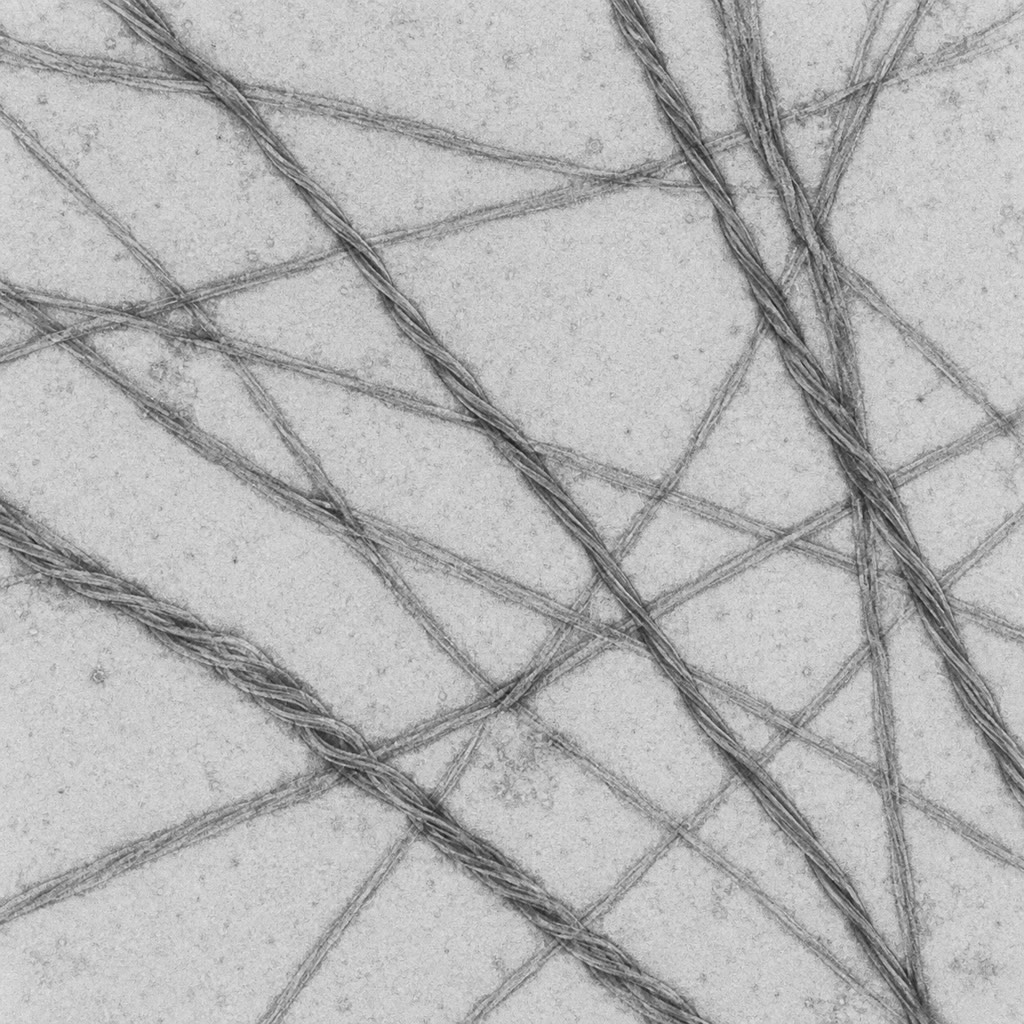
\includegraphics[width=0.36\linewidth]{images/book5/ai/b5-07-amyloid-fibrils.jpg}\hspace{0.04\linewidth}
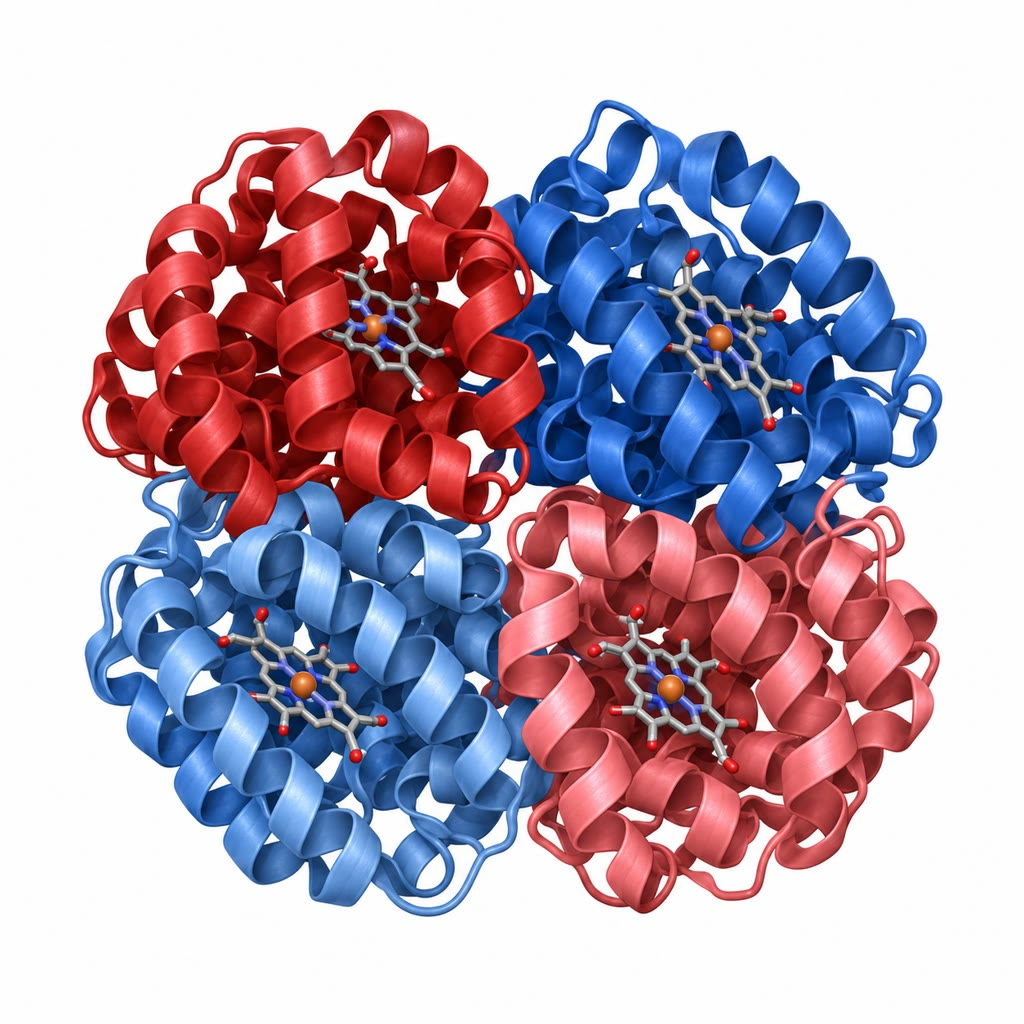
\includegraphics[width=0.36\linewidth]{images/book5/ai/b5-07-haemoglobin-model.jpg}

{\small बाएँ: इलेक्ट्रॉन सूक्ष्मदर्शी में \omterm{def:b3:structural-biology:amyloid}{एमिलॉयड} तंतुक --- सीधे,
अशाखित, कभी-कभी ऐंठे हुए, और वे जिस प्रोटीन के भी बने हों, संरचना में
एक जैसे। दाएँ: हीमोग्लोबिन चतुष्लक, दो $\alpha$ और दो
$\beta$ शृंखलाएँ, हर एक अपने हीम को गोद में लिए।}
\end{omfigure}

\section{किसी प्रोटीन को देखना}

\begin{definition}[संरचनात्मक विधियाँ]\label{def:b3:structural-biology:methods}
\index{X-किरण क्रिस्टलिकी}\index{NMR स्पेक्ट्रमिकी}\index{क्रायो-इलेक्ट्रॉन सूक्ष्मदर्शिकी}\index{विभेदन}
\emph{X-किरण क्रिस्टलिकी} प्रोटीन का कोई क्रिस्टल उगाती है, उसे
X-किरणों के किसी पुंज के सामने रखती है और विवर्तन-प्रतिरूप अंकित करती
है; धब्बों की स्थितियाँ जालक देती हैं और उनकी तीव्रताएँ, तरंगों की
कलाएँ पा लेने के बाद, मात्रक कोष्ठिका का इलेक्ट्रॉन घनत्व देती हैं,
जिसमें शृंखला बनाई जाती है। \emph{नाभिकीय चुंबकीय
अनुनाद} (NMR) विलयन में उन परमाणुओं के नाभिकों के बीच युग्मन मापता है
जो समष्टि में पास-पास हैं, जिनसे दूरियाँ और इसलिए कोई संरचना निकाली
जाती है; यह लगभग \qty{40}{kDa} से छोटे प्रोटीनों के लिए काम करता है
और उनकी गतियाँ बताता है। \emph{क्रायो-इलेक्ट्रॉन सूक्ष्मदर्शिकी}
काचाभ बर्फ़ की किसी पतली झिल्ली में जमे हज़ारों से लाखों अकेले अणुओं
का चित्र लेती है, हर एक किसी यादृच्छिक दिशा में, और उन्हें मिलाकर
त्रिविम घनत्व फिर बनाती है; सीधे इलेक्ट्रॉन संसूचकों (2013) के बाद से
वह परमाण्वीय विभेदन तक पहुँचती है और उसे कोई क्रिस्टल नहीं चाहिए,
इसलिए बड़े संकुल, झिल्ली प्रोटीन और लचीले जमाव, जो कभी क्रिस्टलित नहीं
हुए, अब नियमित रूप से हल किए जाते हैं। किसी संरचना का \emph{विभेदन} वह
सबसे छोटा अंतराल है जिस पर दो लक्षण अलग दिखते हैं:
\qty{0.35}{nm} पर आधार-ढाँचा और बड़ी पार्श्व-शृंखलाएँ रखी जाती हैं,
\qty{0.2}{nm} पर हर परमाणु, \qty{0.1}{nm} पर हाइड्रोजन।
\end{definition}

\begin{proof}[प्रमाण-सामग्री]
केंड्रू (1958) ने किसी प्रोटीन की पहली संरचना पाई, शुक्राणु-व्हेल का
मायोग्लोबिन, \qty{0.6}{nm} पर --- अनपेक्षित अनियमितता वाला एक
सॉसेज, ``किसी के भी पूर्वानुमान से अधिक जटिल और कम सममित''
--- और 1960 में \qty{0.2}{nm} पर, जब पॉलिंग द्वारा 1951 में
प्रतिरूप-रचना से प्रस्तावित $\alpha$-कुंडलियाँ पहली बार देखी गईं।
पेरुत्स (1960) ने हीमोग्लोबिन \qty{0.55}{nm} पर उसी भारी-परमाणु विधि
से हल किया जो उन्होंने कलाएँ पाने के लिए बनाई थी: प्रोटीन से जुड़े
पारद परमाणु तीव्रताएँ ऐसे बदल देते हैं कि छूटी हुई सूचना उजागर हो जाती
है। ऑक्सीजनित और विऑक्सीजनित रूपों की तुलना करते हुए (1970) उन्होंने
देखा कि ऑक्सीजन बँधने पर उपइकाइयाँ एक-दूसरे के सापेक्ष
\qty{15}{\degree} घूम जाती हैं --- परमाण्वीय पैमाने पर देखा गया पहला
अन्यस्थानिक संक्रमण।
\end{proof}

\begin{omfigure}
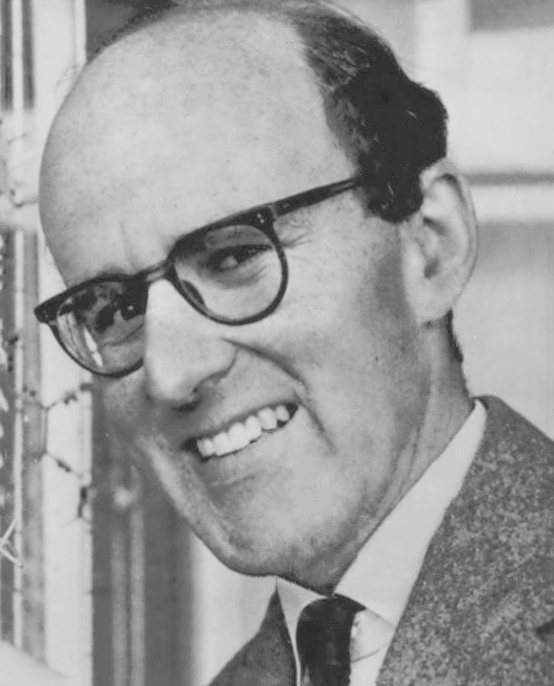
\includegraphics[width=0.30\linewidth]{images/book5/perutz.jpg}\hspace{0.04\linewidth}
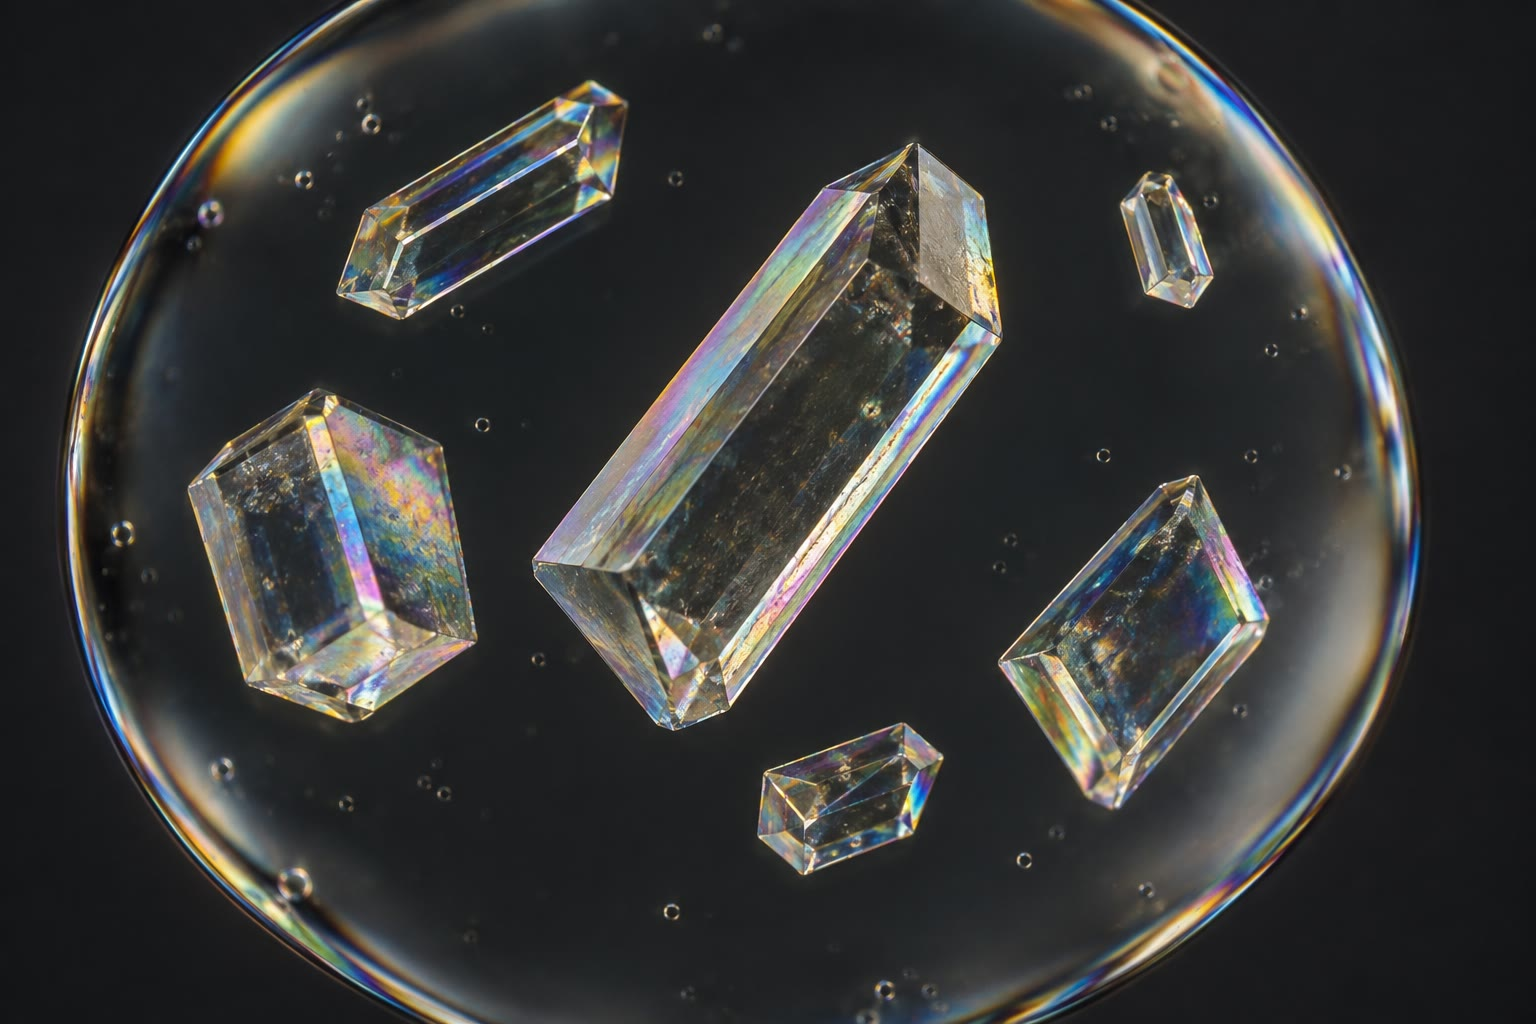
\includegraphics[width=0.30\linewidth]{images/book5/ai/b5-07-protein-crystals.jpg}\hspace{0.04\linewidth}
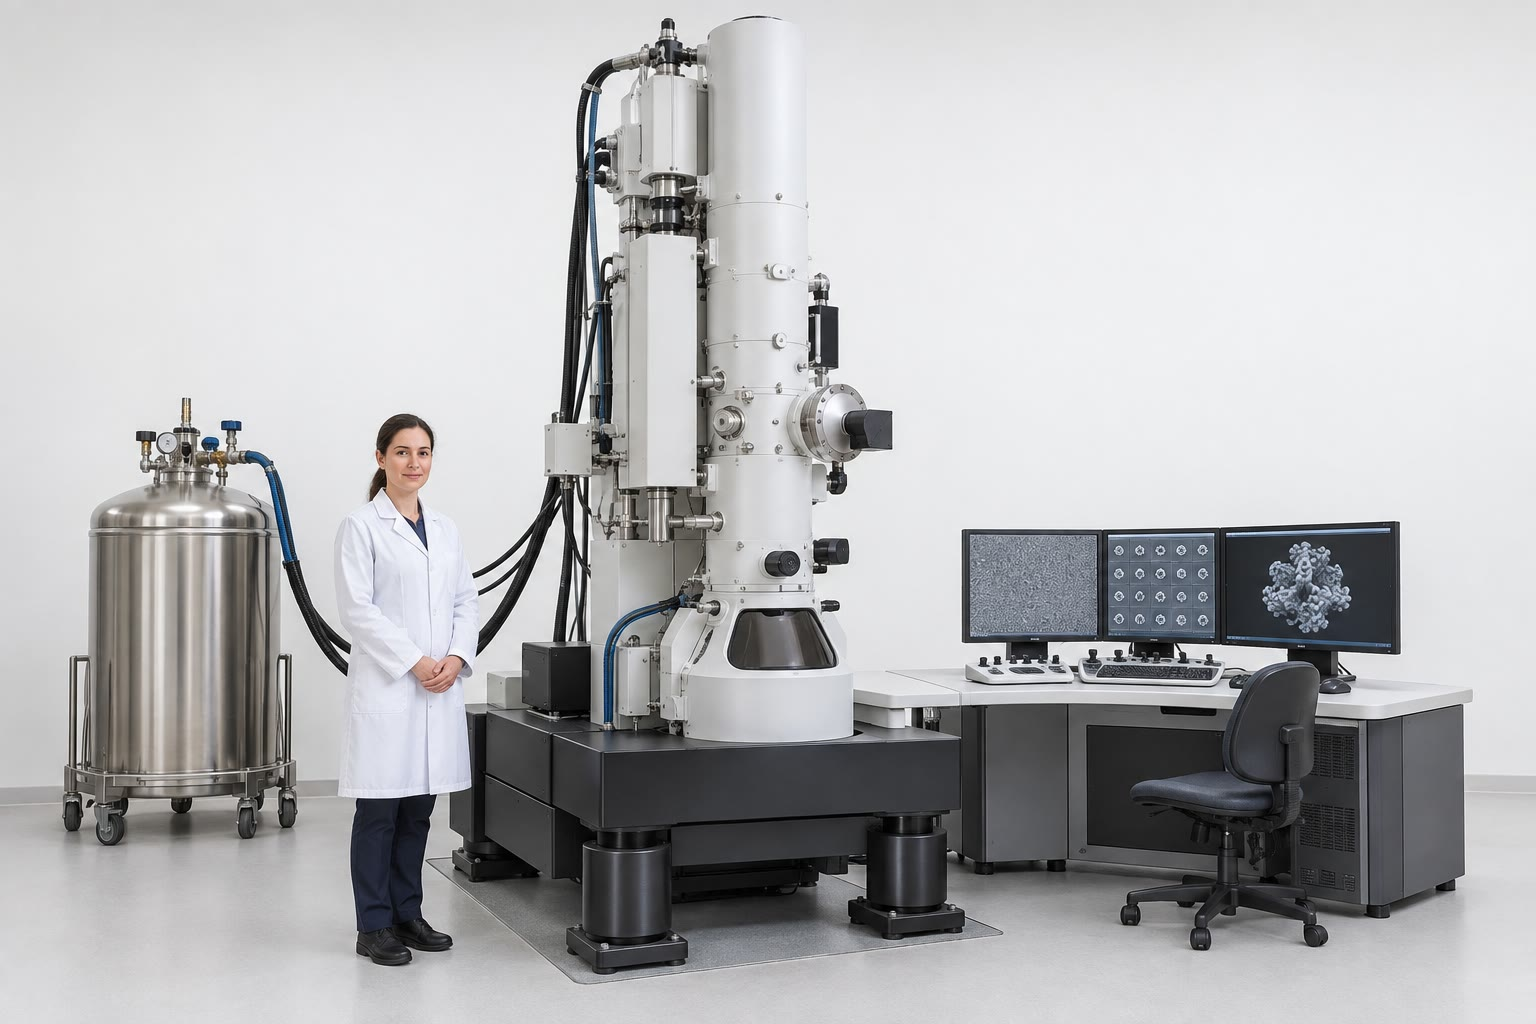
\includegraphics[width=0.30\linewidth]{images/book5/ai/b5-07-cryo-em.jpg}

{\small 1962 में मैक्स पेरुत्स, उसी वर्ष जब उन्हें हीमोग्लोबिन की
संरचना के लिए नोबेल पुरस्कार मिला (असोसिएटेड प्रेस, सार्वजनिक
अधिकार)। बीच में: किसी लटकती बूँद में प्रोटीन क्रिस्टल, क्रिस्टलिकी का
प्रारंभ-बिंदु। दाएँ: कोई क्रायो-इलेक्ट्रॉन सूक्ष्मदर्शी, वह यंत्र
जिसने क्रिस्टलों को अनावश्यक बना दिया।}
\end{omfigure}

\begin{method}[क्रिस्टलिकी से कोई संरचना हल करना]\label{met:b3:structural-biology:crystallography}
\index{ब्रैग का नियम}\index{कला-समस्या}
(1) प्रोटीन के मिलीग्राम भर शुद्ध कीजिए और क्रिस्टलों के लिए सैकड़ों
परिस्थितियाँ (अवक्षेपक, pH, लवण) छानिए; (2) किसी क्रिस्टल को झटपट
जमाइए और किसी सिंक्रोट्रॉन में उसे पुंज में घुमाते हुए विवर्तन-चित्र
लीजिए; (3) मात्रक कोष्ठिका और सममिति पाने के लिए धब्बों की अनुक्रमणिका
बनाइए; जिस अधिकतम कोण पर धब्बे दिखें वह \omterm{met:b3:structural-biology:crystallography}{ब्रैग के नियम} से \omterm{def:b3:structural-biology:methods}{विभेदन} तय कर
देता है, $d =
\lambda/(2\sin\theta)$; (4) \emph{कला-समस्या} हल कीजिए --- संसूचक
तीव्रताएँ अंकित करता है, कलाएँ नहीं --- भारी परमाणुओं से, सेलेनोमेथिओनीन
के सेलेनियम के असामान्य प्रकीर्णन से, या, किसी ज्ञात प्रोटीन से मिलते
प्रोटीन के लिए, आणविक प्रतिस्थापन से, यानी ज्ञात प्रतिरूप को कोष्ठिका
में रखकर; (5) इलेक्ट्रॉन घनत्व निकालिए, उसमें शृंखला बनाइए और आँकड़ों
के सामने प्रतिरूप को तब तक परिष्कृत कीजिए जब तक असहमति
($R$-कारक) छोटी न हो जाए; (6) सत्यापन कीजिए: ज्यामिति, रामचंद्रन
बाह्यमान, और उन आँकड़ों से मेल जिनके सामने प्रतिरूप परिष्कृत नहीं हुआ।
\end{method}

\begin{omfigure}
\begin{tikzpicture}[every node/.style={font=\scriptsize}, >=stealth]
  % crystal
  \draw[thick, fill=omDef!20] (0,0) -- (1.4,0) -- (1.9,0.6) -- (0.5,0.6) -- cycle; \draw[thick, fill=omDef!30] (0,0) -- (0.5,0.6) -- (0.5,1.6) -- (0,1.0) -- cycle; \draw[thick, fill=omDef!25] (0.5,0.6) -- (1.9,0.6) -- (1.9,1.6) -- (0.5,1.6) -- cycle;
  \node[below] at (0.95,-0.1) {क्रिस्टल: पंक्ति में $10^{12}$ अणु};
  % beam
  \draw[->, very thick, omThm] (-2.2,0.9) -- (-0.1,0.9); \node[above] at (-1.2,0.95) {X-किरणें, $\lambda \approx \qty{0.1}{nm}$};
  % diffracted beams
  \foreach \a in {-25,-12,5,18,30} \draw[->, omThm, thick] (1.9,0.9) -- ++(\a:3.2);
  % detector
  \draw[thick] (5.2,-1.2) rectangle (5.6,3.0); \node[right, align=left] at (5.7,2.6) {संसूचक: कोणों $\theta$ पर\\धब्बे, तीव्रताओं\\$I$ के साथ};
  \foreach \y in {-0.6,-0.1,0.6,1.2,1.9,2.4} \fill[black] (5.4,\y) circle (0.06);
  % arrow to density
  \draw[->, very thick] (7.4,0.9) -- (8.6,0.9) node[midway, above, align=center] {कलाएँ\\पा ली गईं};
  \node[right, align=left] at (8.7,1.4) {इलेक्ट्रॉन घनत्व};
  \draw[omDef, thick] (8.8,0.4) .. controls (9.1,1.1) and (9.5,0.2) .. (9.8,0.8) .. controls (10.1,1.3) and (10.4,0.3) .. (10.7,0.9);
  \node[right, align=left] at (8.7,-0.4) {उसमें बनाया, परिष्कृत,\\सत्यापित प्रतिरूप};
  % Bragg
  \node[anchor=north west, align=left] at (-2.2,-0.7) {ब्रैग: $2d\sin\theta = \lambda$ ---\\प्रेक्षित अधिकतम $\theta$ विभेदन $d$ तय करता है};
\end{tikzpicture}

{\small क्रिस्टल से प्रतिरूप तक। नियमित जालक X-किरणों को असतत धब्बों
में प्रकीर्ण करता है; सबसे बड़े कोण वाला धब्बा \omterm{def:b3:structural-biology:methods}{विभेदन} तय करता है;
कलाएँ पा लेने पर तीव्रताएँ किसी इलेक्ट्रॉन-घनत्व मानचित्र में बदल जाती
हैं, जिसमें शृंखला बनाई जाती है।}
\end{omfigure}

\begin{remark}[पूर्वानुमान भी विधियों में आ मिला है]\label{rem:b3:structural-biology:prediction}
2020 से किसी प्रोटीन की संरचना उसके अनुक्रम से ऐसी यथार्थता के साथ
पूर्वानुमानित की जाती है जो प्रायः किसी \qty{0.3}{nm} प्रायोगिक संरचना
की बराबरी करती है (\cref{ch:b3:bioinformatics})। पूर्वानुमान किसी
स्थैतिक प्राकृत अवस्था के बारे में एक परिकल्पना है; प्रायोगिक विधियाँ
ही निर्णायक बनी हुई हैं, और लिगंडों, संरूपणी बदलावों, संकुलों तथा नीचे
चर्चित गतिकी के बारे में सूचना का एकमात्र स्रोत भी। उनकी भूमिकाएँ बदली
हैं --- कोई पूर्वानुमानित प्रतिरूप आणविक प्रतिस्थापन से कला-समस्या हल
कर देता है, और बताता है कि कौन-से प्रयोग करने योग्य हैं --- न कि एक
दूसरे की जगह ले रहा है।
\end{remark}

\section{अन्यस्थानिकता: प्रतिरूप के रूप में हीमोग्लोबिन}

\begin{definition}[अन्यस्थानिकता और सहकारिता]\label{def:b3:structural-biology:allostery}
\index{अन्यस्थानिकता}\index{सहकारिता}\index{हिल गुणांक}\index{T अवस्था}\index{R अवस्था}
कोई प्रोटीन \emph{अन्यस्थानिक} तब है जब किसी एक स्थल पर किसी लिगंड का
बंधन किसी दूसरे स्थल की आसक्ति बदल दे, संरूपता के ऐसे बदलाव द्वारा जो
पूरे अणु में संचरित हो। जब दोनों स्थल एक ही लिगंड से बँधते हों और
प्रभाव धनात्मक हो, तो बंधन \emph{सहकारी} है: भिन्नात्मक संतृप्ति $Y$
लिगंड सांद्रता के साथ किसी अतिपरवलय के बजाय किसी सिग्मॉइड की तरह उठती
है, जिसका अनुभवजन्य वर्णन \emph{हिल समीकरण} $Y = [S]^{n_{H}}/(K^{n_{H}} +
[S]^{n_{H}})$ करता है और जिसमें \emph{हिल गुणांक} $n_{H} > 1$ है
(हीमोग्लोबिन: अपने चार स्थलों के लिए
$n_{H} \approx 2.8$; एक स्थल वाला मायोग्लोबिन: $n_{H} =
1$)। हीमोग्लोबिन दो चतुष्क संरूपताओं में रहता है,
\emph{T अवस्था} (तनी, कम आसक्ति, जो ऑक्सीजन न बँधी हो तब अनुकूल रहती है)
और \emph{R अवस्था} (शिथिल, अधिक आसक्ति), और वह उनके बीच एक इकाई की तरह
बदलता है; प्रोटॉन, कार्बन डाइऑक्साइड और 2,3-द्विफ़ॉस्फ़ोग्लिसरेट T को
स्थिर करते हैं और इस तरह आसक्ति घटाते हैं --- यही \omterm{prop:b3:structural-biology:mechanism}{बोर प्रभाव} है, जिससे
काम करता ऊतक, अम्लीय और गर्म, रक्त से अधिक ऑक्सीजन लेता है।
\end{definition}

\begin{theorem}[मोनो--वाइमन--शांज़ प्रतिरूप]\label{thm:b3:structural-biology:mwc}
\index{मोनो--वाइमन--शांज़ प्रतिरूप}\index{समन्वित प्रतिरूप}
मान लीजिए $n$ समान स्थलों वाला कोई प्रोटीन दो संरूपताओं,
$T$ और $R$, में रहता है, जिनका लिगंड की अनुपस्थिति में साम्य
$L = [T_{0}]/[R_{0}]$ है, $R$ का हर स्थल लिगंड से वियोजन नियतांक
$K_{R}$ के साथ बँधता है और $T$ का हर स्थल $K_{T}$ के साथ,
$c = K_{R}/K_{T} < 1$। किसी अणु के सारे स्थल साथ-साथ बदलते हैं
(संक्रमण \emph{समन्वित} है)। तब $\alpha = [S]/K_{R}$ के साथ
भिन्नात्मक संतृप्ति है
\[
Y = \frac{\alpha(1+\alpha)^{n-1} + Lc\alpha(1+c\alpha)^{n-1}}
{(1+\alpha)^{n} + L(1+c\alpha)^{n}},
\]
और $R$ अवस्था में अणुओं का अंश $\bar R =
(1+\alpha)^{n}/\bigl[(1+\alpha)^{n} + L(1+c\alpha)^{n}\bigr]$ है। $L
\gg 1$ और $c \ll 1$ के लिए वक्र सिग्मॉइड है: पहले लिगंड दुर्लभ,
उच्च-आसक्ति $R$ अणुओं से बँधते हैं और साम्य को झुका देते हैं, जिससे
बंधन और $R$ को बुलाता है और शेष स्थलों की आसक्ति बढ़ जाती है --- स्थलों
के बीच किसी सीधी अन्योन्यक्रिया के बिना \omterm{def:b3:structural-biology:allostery}{सहकारिता}।
\end{theorem}
\begin{proof}
$i$ लिगंड बँधी, $R$ रूप वाली स्पीशीज़ की सांद्रता
$[R_{0}]\binom{n}{i}\alpha^{i}$ है (अधिकृत स्थलों के $\binom{n}{i}$
चुनावों में से हर एक द्रव्यमान-क्रिया के नियम से $([S]/K_{R})^{i}$
देता है), और $T$ रूप में $[T_{0}]\binom{n}{i}(c\alpha)^{i}$, क्योंकि
$[S]/K_{T} = c\alpha$ है। द्विपद प्रमेय से $i$ पर योग लेने पर कुल
प्रोटीन $[R_{0}]\bigl[(1+\alpha)^{n} + L(1+c\alpha)^{n}\bigr]$ है
और कुल बँधा लिगंड $[R_{0}]\sum_{i} i\binom{n}{i}\bigl[
\alpha^{i} + L(c\alpha)^{i}\bigr] = [R_{0}]\,n\bigl[\alpha(1+\alpha)^{n-1}
+ Lc\alpha(1+c\alpha)^{n-1}\bigr]$, जिसमें $\sum_{i} i\binom{n}{i}x^{i} =
nx(1+x)^{n-1}$ काम में आया है। बँधे लिगंड को $n$ गुना कुल प्रोटीन से
भाग देने पर $Y$ मिलता है; $R$ अंश कुल पर $R$ पदों का अनुपात है। जब
$\alpha$ छोटा हो तो हर में $T$ पदों का बोलबाला रहता है (क्योंकि $L \gg 1$)
और $Y \approx c\alpha$, यानी नीची $T$ आसक्ति; जब $\alpha$ इतना बड़ा
हो कि $(1+\alpha)^{n} > L(1+c\alpha)^{n}$ हो जाए तो $R$ पद ले लेते हैं
और आसक्ति $K_{R}$ है: दोनों प्रांतों के बीच का यही स्विच सिग्मॉइड है।
\end{proof}

\begin{example}[संख्याओं में हीमोग्लोबिन]\label{ex:b3:structural-biology:hb-numbers}
$n = 4$, $K_{R} = \qty{1}{mmHg}$, $c = 0.01$ (इसलिए $K_{T} =
\qty{100}{mmHg}$) और $L = 3\times 10^{5}$ लीजिए। धमनी रक्त में
ऑक्सीजन के आंशिक दाब, \qty{100}{mmHg}, पर $\alpha = 100$ और $Y =
0.97$; \qty{40}{mmHg} पर, जो विश्राम का शिरा-मान है, $Y = 0.78$;
\qty{26}{mmHg} पर $Y = 0.52$ --- प्रतिरूप \qty{26}{mmHg} का
अर्ध-संतृप्ति दाब फिर से दे देता है; किसी व्यायाम करती पेशी में
\qty{20}{mmHg} पर $Y = 0.35$। उसी अर्ध-संतृप्ति दाब वाला कोई असहकारी
वाहक फेफड़ों में $100/126 = 0.79$ और पेशी में
$20/46 = 0.43$ देता, यानी अपनी क्षमता का $0.36$ उतारता, जहाँ
हीमोग्लोबिन $0.62$ उतारता है। \omterm{def:b3:structural-biology:allostery}{सहकारिता} ही ऐसा वाहक बनाती है जो एक दाब
पर पूरा भर जाए और केवल पाँच गुना नीचे के दाब पर अधिकांश उतार दे।
\end{example}

\begin{omfigure}
\begin{tikzpicture}
\begin{axis}[
  width=0.7\linewidth, height=5.8cm,
  axis x line=bottom, axis y line=left,
  xmin=0, xmax=120, ymin=0, ymax=1.05,
  xlabel={ऑक्सीजन आंशिक दाब (mmHg)}, ylabel={संतृप्ति $Y$},
  xlabel style={font=\small, at={(axis description cs:0.5,-0.12)}, anchor=north},
  ylabel style={font=\small},
  tick label style={font=\small}, xtick={0,20,40,60,80,100,120}, ytick={0,0.5,1},
  clip=false,
]
\addplot[very thick, omThm, domain=0.1:120, samples=120] {(x*(1+x)^3 + 300000*0.01*x*(1+0.01*x)^3)/((1+x)^4 + 300000*(1+0.01*x)^4)};
\addplot[very thick, omDef, domain=0:120, samples=60] {x/(x+26)};
\addplot[dashed, gray] coordinates {(26,0) (26,0.52)}; \addplot[dashed, gray] coordinates {(0,0.52) (26,0.52)};
\draw[gray, dashed] (axis cs:20,0) -- (axis cs:20,0.35); \draw[gray, dashed] (axis cs:100,0) -- (axis cs:100,0.97);
\node[font=\scriptsize, omThm, anchor=north west] at (axis cs:50,0.15) {हीमोग्लोबिन (MWC, $n = 4$, $L = 3\times 10^{5}$, $c = 0.01$)};
\node[font=\scriptsize, omDef, anchor=north east] at (axis cs:118,0.72) {एक स्थल, वही $P_{50}$};
\node[font=\scriptsize, anchor=south] at (axis cs:20,1.0) {पेशी}; \node[font=\scriptsize, anchor=south] at (axis cs:100,1.0) {फेफड़ा};
\end{axis}
\end{tikzpicture}

{\small उदाहरण के प्राचलों के साथ मोनो--वाइमन--शांज़ समीकरण से निकाली
गई हीमोग्लोबिन की ऑक्सीजन संतृप्ति (लाल), उसी अर्ध-संतृप्ति दाब वाले
किसी एक-स्थल वाहक (नीला) के सामने। फेफड़े और काम करती पेशी के बीच
सहकारी वाहक लगभग दोगुना उतारता है।}
\end{omfigure}

\begin{proposition}[स्विच की क्रियाविधि]\label{prop:b3:structural-biology:mechanism}
\index{बोर प्रभाव}\index{2,3-द्विफ़ॉस्फ़ोग्लिसरेट}
विऑक्सीहीमोग्लोबिन में लोहा हीम-तल से थोड़ा बाहर बैठता है, समीपस्थ
हिस्टिडीन की ओर खिंचा हुआ, और हीम गुंबदाकार होता है। ऑक्सीजन का बंधन
हीम को चपटा कर देता है और लोहे को, और उसके साथ हिस्टिडीन तथा उस कुंडली
को जिसका वह अंग है, लगभग \qty{0.06}{nm} हीम की ओर खींच लेता है; वह
खिसकाव $\alpha_{1}\beta_{1}$ और $\alpha_{2}\beta_{2}$ द्विलकों के बीच
की अंतराफलक पर प्रवर्धित होता है, जो \qty{15}{\degree} घूम जाते हैं और
उन लवण-सेतुओं को तोड़ देते हैं जो \omterm{def:b3:structural-biology:allostery}{T अवस्था} थामे रहते हैं।
प्रभावक उन्हीं सेतुओं पर काम करते हैं: प्रोटॉन ऐसे हिस्टिडीनों से
बँधते हैं जिनके सेतु केवल T में हैं (\omterm{prop:b3:structural-biology:mechanism}{बोर प्रभाव}), कार्बन डाइऑक्साइड
अमीनो सिरों के साथ कार्बामेट बनाता है जो T को स्थिर करते हैं, और
2,3-द्विफ़ॉस्फ़ोग्लिसरेट, एक तीव्र ऋणात्मक छोटा अणु, $\beta$
शृंखलाओं के बीच की केंद्रीय गुहा में बैठता है, जो केवल T में इतनी चौड़ी
होती है। भ्रूणीय हीमोग्लोबिन, जिसकी $\gamma$ शृंखलाएँ उससे कम अच्छी तरह
बँधती हैं, माता के हीमोग्लोबिन से अधिक आसक्ति रखता है और अपरा के पार
ऑक्सीजन खींच लेता है।
\end{proposition}

\section{गतिमान प्रोटीन}

\begin{definition}[अव्यवस्था और गतिकी]\label{def:b3:structural-biology:disorder}
\index{स्वाभाविक अव्यवस्थित प्रोटीन}\index{संरूपणी समुदाय}\index{जैव-आणविक संघनित}
किसी \emph{स्वाभाविक रूप से अव्यवस्थित} क्षेत्र का अपने आप कोई स्थिर
\omterm{def:b3:structural-biology:levels}{वलन} नहीं होता और वह तेज़ी से आपस में बदलती संरूपताओं के किसी समुदाय के
रूप में रहता है, और प्रायः तभी वलित होता है जब वह अपने साथी से मिले;
लगभग एक-तिहाई मानव प्रोटीन तीस से अधिक अवशेषों का कोई अव्यवस्थित
क्षेत्र ढोते हैं, और वे संकेतन तथा नियमन में बहुतायत से हैं, जहाँ कोई
लचीला खंड अनेक स्थलों पर फ़ॉस्फ़ोरिलित हो सकता है, बारी-बारी से कई
साथियों से बँध सकता है, और किसी योजक का काम कर सकता है। वलित प्रोटीन भी
चलते हैं: पार्श्व-शृंखलाएँ पिकोसेकंडों में घूमती हैं, फंदे नैनोसेकंडों
से माइक्रोसेकंडों में खुलते हैं, \omterm{def:b3:structural-biology:levels}{प्रांत} माइक्रोसेकंडों से
मिलीसेकंडों में कब्ज़े की तरह मुड़ते हैं, और किसी एंज़ाइम का उत्प्रेरक
चक्र किसी स्थैतिक ताला-कुंजी के बजाय ऐसी ही गतियों का नृत्य है। कोई
क्रिस्टल संरचना किसी \emph{संरूपणी समुदाय} का एक चित्र है; शेष NMR और
आणविक अनुरूपण देखते हैं। बहुसंयोजी अव्यवस्थित प्रोटीन और RNA
कोशिकाद्रव्य से अलग होकर तरल बूँदों में भी जम सकते हैं ---
\emph{जैव-आणविक संघनित} जैसे केंद्रिकाएँ, तनाव कणिकाएँ और P पिंड ---
जो बिना किसी झिल्ली के अभिक्रियाएँ सांद्र कर देते हैं, और जिनका बूढ़े
होकर ठोस पुंजों में बदल जाना \omterm{def:b3:structural-biology:amyloid}{एमिलॉयड} रोगों का एक मार्ग है।
\end{definition}

\begin{remark}[संरचना और प्रकार्य]\label{rem:b3:structural-biology:sf}
साठ वर्षों की संरचनाओं का पाठ दोहरा है। कोई \omterm{def:b3:structural-biology:levels}{वलन} किसी भौतिक समस्या का
समाधान है --- इसे बाँधो, उसका उत्प्रेरण करो, कोई संकेत चार नैनोमीटर पार
पहुँचाओ --- और संरचना जान लेने से क्रियाविधि प्रायः स्पष्ट हो जाती है,
जैसे हीम के लोहे के लिए और हीमोग्लोबिन के द्विलकों के ऑक्सीजन-चालित
घूर्णन के लिए हुई। और कोई \omterm{def:b3:structural-biology:levels}{वलन} एक ऐतिहासिक वस्तु है: वही कुछ सौ
स्थापत्य, जिन्हें छेड़ा, द्विगुणित और संलयित किया गया है, प्रोटीन
प्रकार्य की पूरी विविधता के काम आते हैं, जिससे किसी जीवाणु के प्रोटीन
की संरचना प्रायः बता देती है कि मानव चचेरा भाई कैसे काम करता है।
\end{remark}

\section{अभ्यास}

\begin{exercise}[$\star$]\label{exo:b3:structural-biology:1}
प्रोटीन संरचना के चारों स्तर परिभाषित कीजिए और हीमोग्लोबिन में हर एक का
उदाहरण दीजिए।
\end{exercise}

\begin{exercise}[$\star$]\label{exo:b3:structural-biology:2}
किसी $\alpha$-कुंडली में $36$ अवशेष हैं। वह कितनी लंबी है, कितने फेरे
लेती है, और कितने आधार-ढाँचा हाइड्रोजन बंध उसे थामे रहते हैं (हर अवशेष
का कार्बोनिल चार अवशेष आगे के एमाइड से बँधता है)?
\end{exercise}

\begin{exercise}[$\star$]\label{exo:b3:structural-biology:3}
ऐनफ़िन्सन के राइबोन्यूक्लिएज़ पुनर्वलन ने क्या दिखाया, और प्रयोग को
किसी भी कोशिकीय अंग की अनुपस्थिति में करना क्यों महत्वपूर्ण था?
\end{exercise}

\begin{exercise}[$\star$]\label{exo:b3:structural-biology:4}
क्रिस्टलिकी, NMR और \omterm{def:b3:structural-biology:methods}{क्रायो-इलेक्ट्रॉन सूक्ष्मदर्शिकी} को उस प्रोटीन-आकार
के क्रम में रखिए जिसे हर एक सबसे अच्छी तरह सँभालती है, और बताइए कि
कौन-सी गति के बारे में सूचना देती है।
\end{exercise}

\begin{exercise}[$\star\star$]\label{exo:b3:structural-biology:5}
$150$ अवशेषों के किसी प्रोटीन के लिए, $k = 2$ के साथ, और
$20$ अवशेषों के किसी पेप्टाइड के लिए, $k = 3$ के साथ, लेविंथल की गिनती
फिर से कीजिए। इन
दोनों में से किसके लिए प्रति सेकंड $10^{12}$ प्रयासों पर एक सेकंड के
भीतर कोई यादृच्छिक खोज सोची जा सकती है?
\end{exercise}

\begin{exercise}[$\star\star$]\label{exo:b3:structural-biology:6}
$n = 2$, $L = 100$, $c = 0.01$ के साथ MWC समीकरण का उपयोग करते हुए
$Y$ निकालिए, $\alpha = 1$, $10$ और $100$ पर, और वियोजन नियतांक
$K_{R}$ वाले किसी एक स्थल ($Y = \alpha/(1+\alpha)$) से तुलना कीजिए।
\omterm{def:b3:structural-biology:allostery}{सहकारिता} कहाँ दिखती है?
\end{exercise}

\begin{exercise}[$\star\star$]\label{exo:b3:structural-biology:7}
MWC प्रतिरूप से समझाइए कि 2,3-द्विफ़ॉस्फ़ोग्लिसरेट हीमोग्लोबिन की
ऑक्सीजन-आसक्ति क्यों घटाता है, वह प्रतिरूप का कौन-सा प्राचल बदलता है,
और संचित रक्त, जो यह यौगिक खो देता है, आधान करने पर ऑक्सीजन खराब ढंग
से क्यों पहुँचाता है।
\end{exercise}

\begin{exercise}[$\star\star$]\label{exo:b3:structural-biology:8}
कोई क्रिस्टल \qty{0.1}{nm} तरंगदैर्घ्य की X-किरणों के साथ अधिकतम कोण
$\theta = \qty{15}{\degree}$ तक विवर्तन देता है। \omterm{def:b3:structural-biology:methods}{विभेदन} क्या है?
प्रोटीन के कौन-से लक्षण दिखेंगे? \qty{0.12}{nm} के लिए कौन-सा कोण
चाहिए होता?
\end{exercise}

\begin{exercise}[$\star\star$]\label{exo:b3:structural-biology:9}
कोई उत्परिवर्तन किसी दबे हुए ल्यूसीन की जगह कोई लाइसीन रख देता है।
\cref{prop:b3:structural-biology:forces} का उपयोग करते हुए स्थायित्व पर
उसके प्रभाव का पूर्वानुमान कीजिए, और समझाइए कि वही प्रतिस्थापन पृष्ठ पर
क्यों हानिरहित होता। फिर समझाइए कि $\Delta G_{\text{वलन}} =
\qty{-30}{kJ/mol}$ वाला कोई प्रोटीन ``बहुत स्थिर'' क्यों नहीं है,
यद्यपि संख्या बड़ी दिखती है।
\end{exercise}

\begin{exercise}[$\star\star\star$]\label{exo:b3:structural-biology:10}
\cref{thm:b3:structural-biology:mwc} के प्रमाण में गिनी गई स्पीशीज़ से
$R$ अवस्था में अणुओं का अंश, $\bar R$, व्युत्पन्न कीजिए,
और दिखाइए कि $c \to 0$ के लिए वह लिगंड सांद्रता जिस पर आधे अणु
$R$ में हों, $(1+\alpha)^{n} = L$ का पालन करती है। हीमोग्लोबिन के
प्राचलों के लिए यह $\alpha$ निकालिए और $P_{50}$ से तुलना कीजिए।
\end{exercise}

\begin{exercise}[$\star\star\star$]\label{exo:b3:structural-biology:11}
\omterm{def:b3:structural-biology:amyloid}{प्रायॉन} कोई आकार संचरित करते हैं। समझाइए कि ``केवल-प्रोटीन'' परिकल्पना
का विरोध क्यों हुआ, कौन-सा प्रयोग उसका खंडन करेगा, और कौन-से प्रमाण
(न्यूक्लिएज़ों तथा पराबैंगनी प्रकाश के प्रति संक्राम्यता का प्रतिरोध,
प्रोटीन विकृतकों के प्रति संवेदिता, संश्लेषित \omterm{def:b3:structural-biology:amyloid}{प्रायॉन}) उसका समर्थन करते
हैं। किसी \omterm{def:b3:structural-biology:amyloid}{प्रायॉन} को कोई बीज क्यों चाहिए?
\end{exercise}

\begin{exercise}[$\star\star\star$]\label{exo:b3:structural-biology:12}
किसी प्रोटीन कुल ने अपना \omterm{def:b3:structural-biology:levels}{वलन} बनाए रखा है जबकि उसके अनुक्रम \qty{15}{\%}
समरूपता तक अपसरित हो चुके हैं। समझाइए कि संरचना अनुक्रम से अधिक
संरक्षित क्यों है, कौन-से अवशेष संरक्षित रहते हैं, और इसका उपयोग
प्रोफ़ाइल विधियाँ (\cref{ch:b3:bioinformatics}) तथा नए प्रोटीनों का
अभिकल्प दोनों कैसे करते हैं।
\end{exercise}

\section{समस्या: किसी ग्लोबिन का वलन}

\begin{problem}[{सप्तांत समस्या --- किसी ग्लोबिन की कुंडलियाँ मापी गईं,
उसका वलन लेविंथल के सामने समयबद्ध किया गया, उसका ऑक्सीजन-बंधन
द्वि-अवस्था प्रतिरूप से निकाला गया, और उसकी संरचना किसी क्रिस्टल से हल
की गई, जिसका अंत फेफड़े और पेशी के बीच संतृप्ति-अंतर, लेविंथल-काल और
मानचित्र के विभेदन पर होता है}]
\label{pb:b3:structural-biology:1}
आँकड़े: $150$ अवशेषों की कोई ग्लोबिन शृंखला, माध्य अवशेष-द्रव्यमान \qty{110}{Da},
अवशेषों का \qty{75}{\%} आठ $\alpha$-कुंडलियों में; कुंडली का उठान
प्रति अवशेष \qty{0.15}{nm}, प्रति फेरा $3.6$ अवशेष। प्रोटीन का आंशिक
विशिष्ट आयतन \qty{0.73}{cm^3/g}। हीमोग्लोबिन के लिए MWC प्राचल:
$n = 4$, $K_{R} = \qty{1}{mmHg}$, $c = 0.01$, $L = 3\times 10^{5}$।
X-किरण तरंगदैर्घ्य \qty{0.1}{nm}; मात्रक कोष्ठिका \qty{6}{nm} भुजा का घन;
क्रिस्टल \qty{100}{\micro m} भुजा का घन।

\medskip
\noindent\textbf{भाग I --- किसी शृंखला की शारीरिकी।}
\begin{enumerate}
  \item कुंडलियों में कितने अवशेष हैं? वह कितनी कुल कुंडली-लंबाई हुई,
        और कितने फेरे?
  \item कुंडलियाँ कितने आधार-ढाँचा हाइड्रोजन बंध रखती हैं, हर कुंडली
        के पहले चार अवशेषों के आगे प्रति अवशेष एक गिनते हुए?
  \item शृंखला का द्रव्यमान और आंशिक विशिष्ट आयतन से उसका आयतन; उस
        आयतन के किसी गोले की त्रिज्या।
  \item फैली हुई शृंखला प्रति अवशेष \qty{0.36}{nm} लंबी होती।
        उसकी लंबाई की गोले के व्यास से तुलना कीजिए: \omterm{def:b3:structural-biology:levels}{वलन} शृंखला को
        किस गुणक से सघन करता है?
  \item आठों कुंडलियाँ औसतन $14$ अवशेषों की हैं। यदि अवशेष सिरे से
        सिरा मिलाकर रखे जाएँ, तो फैली हुई लंबाई का कितना अंश कुंडलित
        है, और कुंडली उसे कैसे छोटा करती है?
  \item कोई ग्लोबिन अपने क्रोड में लगभग $40$ अध्रुवी पार्श्व-शृंखलाएँ
        दबाता है। प्रति दबी पार्श्व-शृंखला \qty{4}{kJ/mol} जलविरोधी
        स्थिरीकरण और \omterm{def:b3:structural-biology:levels}{वलन} पर प्रति अवशेष (सभी $150$)
        \qty{0.9}{kJ/mol} की संरूपणी एन्ट्रॉपी-लागत लेकर
        \omterm{def:b3:structural-biology:levels}{वलन} का शुद्ध $\Delta G$ आँकिए और
        \cref{prop:b3:structural-biology:forces} के परास से तुलना कीजिए।
\end{enumerate}

\medskip
\noindent\textbf{भाग II --- \omterm{def:b3:structural-biology:levels}{वलन} ढूँढ़ना।}
\begin{enumerate}[resume]
  \item $150$ अवशेषों के लिए, $k = 3$ के साथ, लेविंथल की गिनती और
        उसे प्रति सेकंड $10^{12}$ की दर से छानने का समय निकालिए।
  \item ग्लोबिन \qty{10}{ms} में वलित होता है। वह अधिक-से-अधिक कितनी
        संरूपताएँ देख सकता है? वह गिनती का कितना अंश है?
  \item इसके बजाय मान लीजिए हर कुंडली स्वतंत्र रूप से
        \qty{1}{\micro s} में बनती है, और फिर आठों बनी कुंडलियाँ अपना
        जमाव $8!$ क्रमों में से प्रति सेकंड $10^{6}$ की दर से छानकर
        ढूँढ़ती हैं। वलन-काल आँकिए। क्या यह कोई कीप है?
  \item कोई \omterm{def:b3:structural-biology:chaperones}{अनुरक्षकी} प्रति चक्र \qty{10}{s} तक किसी शृंखला को बंद
        रखती है और उसे प्रति चक्र प्रायिकता $0.3$ से वलित छोड़ती है।
        किसी कठिन क्रियाधार को वलित करने के लिए चक्रों की प्रत्याशित
        संख्या और प्रत्याशित समय क्या है? एक मिनट बाद कितना अंश अब भी
        अवलित है?
  \item कोई अस्थिरकारी उत्परिवर्तन \qty{37}{\celsius} पर अवलित अंश
        $10^{-4}$ से बढ़ाकर $10^{-2}$ कर देता है। $\Delta G =
        -RT\ln(K)$ और $K = [\text{वलित}]/[\text{अवलित}]$ के साथ
        $\Delta G_{\text{वलन}}$ कितना बदला?
  \item बीज की आवश्यकता का उपयोग करते हुए समझाइए कि सौ गुना अधिक अवलित
        प्रोटीन स्वास्थ्य और \omterm{def:b3:structural-biology:amyloid}{एमिलॉयड} रोग के बीच का अंतर क्यों हो सकता
        है।
\end{enumerate}

\medskip
\noindent\textbf{भाग III --- ऑक्सीजन बाँधना।}
\begin{enumerate}[resume]
  \item MWC समीकरण से $Y$ निकालिए, $\alpha = 100$ (फेफड़ा) और
        $\alpha = 20$ (काम करती पेशी) पर।
  \item उन्हीं दो दाबों पर $R$ अवस्था में अणुओं का अंश निकालिए।
  \item फेफड़े और पेशी के बीच भरी हुई ऑक्सीजन का कितना भाग उतरता है?
        \qty{26}{mmHg} अर्ध-संतृप्ति दाब वाले किसी एक-स्थल वाहक से
        तुलना कीजिए।
  \item रक्त प्रति लीटर \qty{150}{g} हीमोग्लोबिन ढोता है, और हर ग्राम
        \qty{1.34}{mL} ऑक्सीजन बाँधता है। प्रश्न 15 से, हीमोग्लोबिन
        प्रति लीटर कितने मिलीलीटर ऑक्सीजन पेशी तक पहुँचाता है? कोई
        विश्राम करता शरीर \qty{250}{mL/min} खपाता है: विश्राम में उसके
        लिए कितना रक्त-प्रवाह चाहिए ($0.97$ से $0.78$ तक उतारते हुए)?
  \item द्विफ़ॉस्फ़ोग्लिसरेट $L$ को $3\times 10^{6}$ तक उठा देता है।
        $Y$ फिर से निकालिए, $\alpha = 40$ पर, और बताइए कि विश्राम में
        इससे पहुँच पर क्या असर पड़ता है।
  \item भ्रूणीय हीमोग्लोबिन का, प्रभाव की दृष्टि से, $L = 3\times 10^{4}$
        है। \qty{30}{mmHg} के अपरा-दाब पर उसका $Y$ निकालिए, माता के
        साथ तुलना कीजिए, और स्थानांतरण समझाइए।
\end{enumerate}

\medskip
\noindent\textbf{भाग IV --- उसे देखना।}
\begin{enumerate}[resume]
  \item क्रिस्टल में कितनी मात्रक कोष्ठिकाएँ हैं? यदि हर कोष्ठिका में
        चार ग्लोबिन शृंखलाएँ हों, तो कितने अणु साथ विवर्तन देते हैं?
  \item धब्बे $\theta = \qty{14.5}{\degree}$ तक दिखते हैं। \omterm{def:b3:structural-biology:methods}{विभेदन} क्या
        है, और क्या पार्श्व-शृंखलाएँ रखी जा सकेंगी?
  \item \qty{0.15}{nm} के लिए कौन-सा कोण चाहिए? किसी बुरी तरह क्रमित
        क्रिस्टल का विवर्तन केवल छोटे कोणों तक क्यों जाता है?
  \item \omterm{def:b3:structural-biology:methods}{क्रायो-इलेक्ट्रॉन सूक्ष्मदर्शिकी} में औसत किए गए चित्र का संकेत
        कणों की संख्या के वर्गमूल की तरह बढ़ता है। यदि
        \num{10000} कण \qty{0.6}{nm} दें, और \omterm{def:b3:structural-biology:methods}{विभेदन} संकेत के व्युत्क्रम
        की तरह सुधरे, तो \qty{0.3}{nm} के लिए कितने कण चाहिए?
  \item \omterm{def:b3:structural-biology:methods}{क्रायो-इलेक्ट्रॉन सूक्ष्मदर्शिकी} को कोई क्रिस्टल नहीं चाहिए।
        दो ऐसे प्रकार के प्रोटीन या संकुल बताइए जिनके लिए यह तय करता
        है कि कोई संरचना मिल भी सकेगी या नहीं, और कारण समझाइए।
  \item ग्लोबिन का कोई पूर्वानुमानित प्रतिरूप क्रिस्टल संरचना से
        आधार-ढाँचे पर औसतन \qty{0.1}{nm} भिन्न है। दो ऐसी बातें
        बताइए जो पूर्वानुमान नहीं दे सकता पर क्रिस्टल ने दीं।
  \item सारांश दीजिए: फेफड़े और पेशी के बीच उतराई (प्रश्न~15),
        $150$ अवशेषों के लिए लेविंथल-काल (प्रश्न~7), और मानचित्र का
        \omterm{def:b3:structural-biology:methods}{विभेदन} (प्रश्न~20)।
\end{enumerate}
\end{problem}
